\newpage
\section{Monitorowanie działania systemu}
Monitorowanie działania systemu realizowane było  za pomocą zbierania i analizy logów. W celu ułatwienia analizy,  został utworzony panel do obserwacji. Panel taki można wykonać za pomocą narzędzia - Kibana. Narzędzie to ma wiele możliwości, takich jak przeszukiwanie istniejących logów czy tworzenie paneli. Przeszukania  aktualnych logów dokonujemy przy użyciu widoku Discover, w którym możliwe jest  wyszukanie logów na podstawie nazw kontenera z którego pochodzą, na podstawie frazy w nich zawartej, ich daty, czy wielu innych parametrów:
\begin{figure}[H]
    \centering
    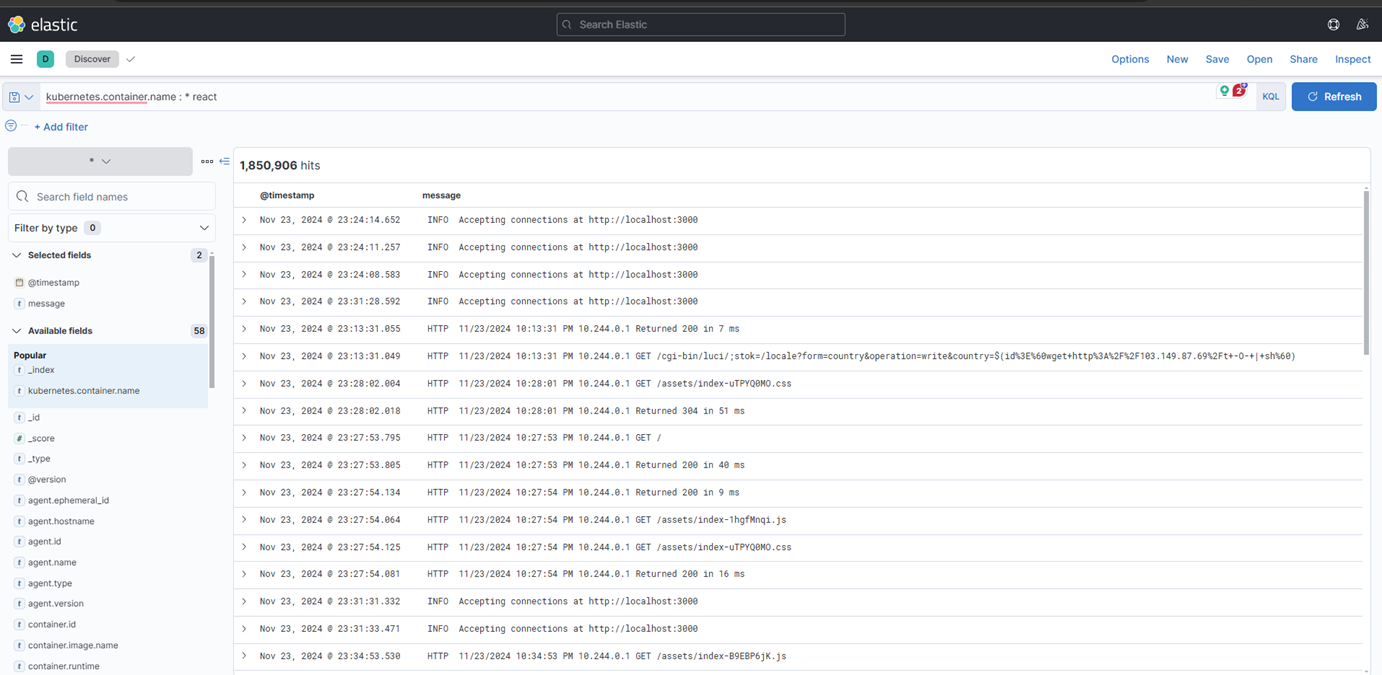
\includegraphics[width=1\linewidth]{logs_view.png}
    \caption{Wyświetlenie logów w kibanie}
    \label{fig:kibana-logs}
\end{figure}

Dzięki wbudowanym w narzędzie Kibana modułu do analiz, możemy wytworzyć analizy całości logów. Na analizie przedstawionej poniżej,  w pierwszej sekcji od góry znajdują się aktualne logi, następnie poniżej, licząc od lewej: liczba wszystkich logów, liczba logów informujących o error'ach oraz stosunek tych ostatnich względem sumy wszystkich. W ostatnim rzędzie prezentowane są  wykresy obrazujące: które kontenery pokazują najwięcej logów związanych z error'ami oraz jak zapis logów w czasie. Dla dokładniejszej wizualizacji, można dowolnie dobrać przedział czasowy do prezentacji danych.
\begin{figure}[H]
    \centering
    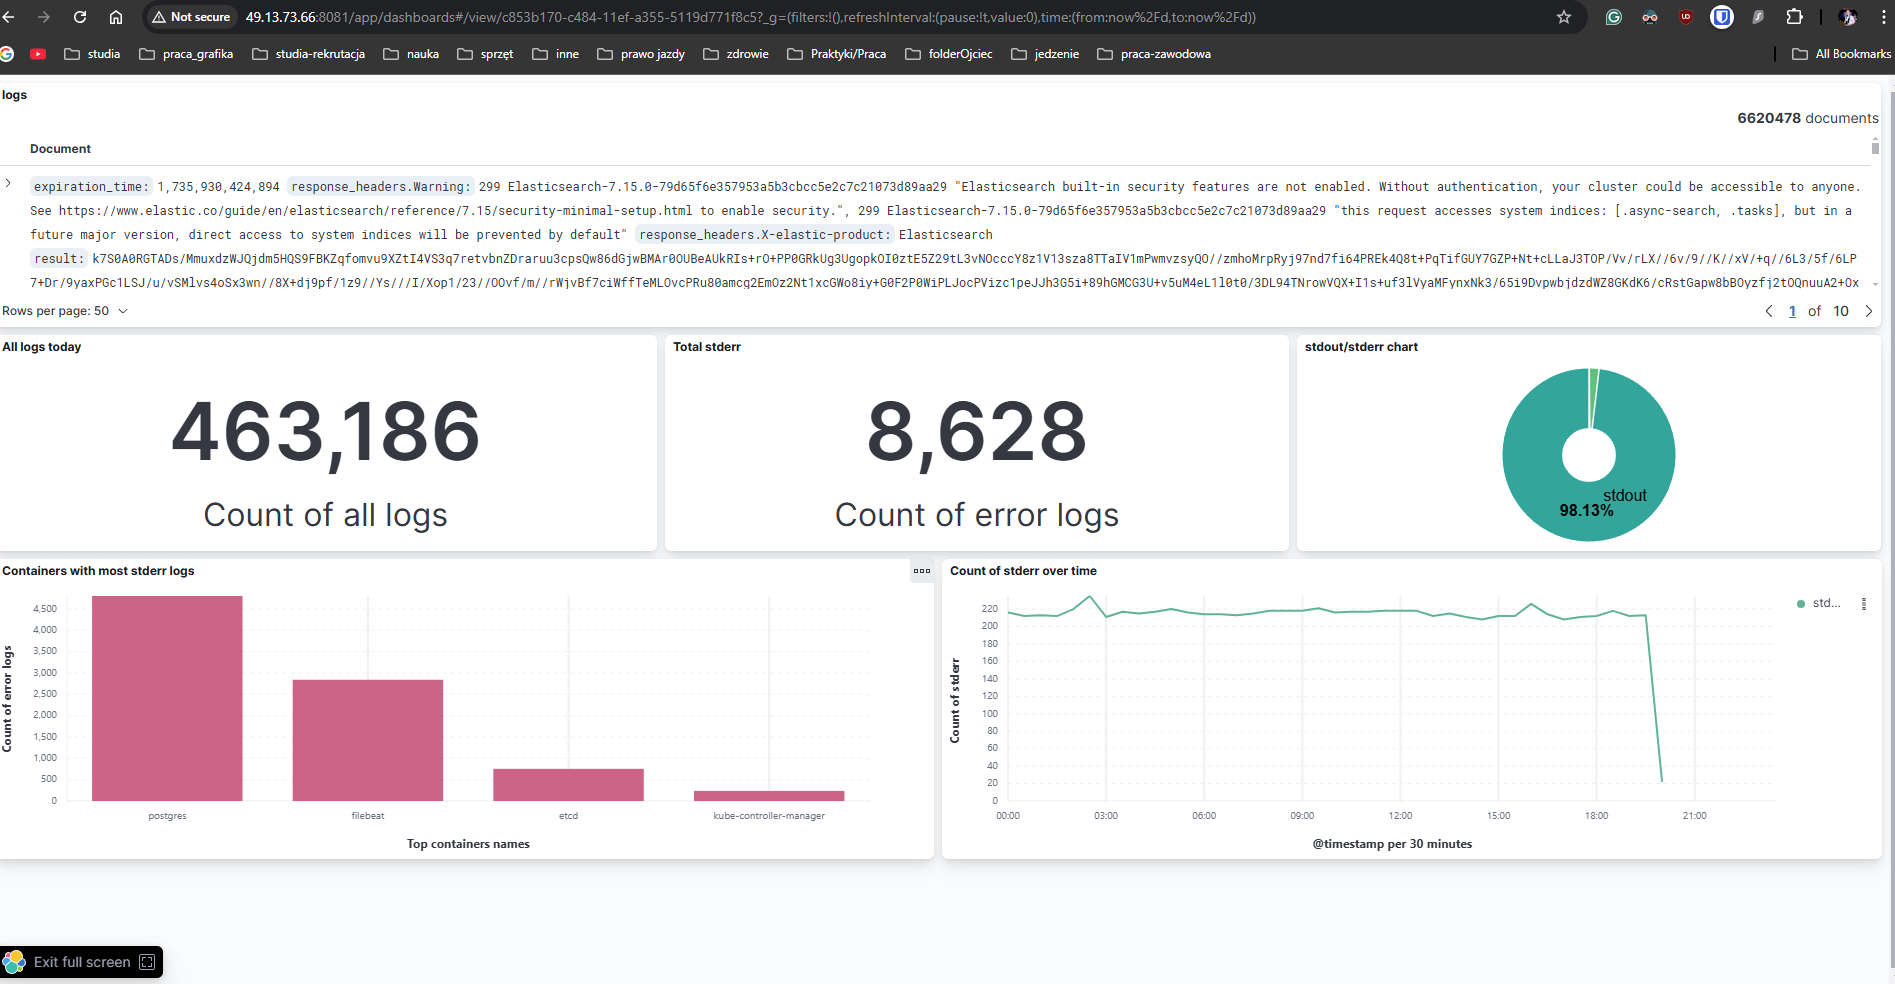
\includegraphics[width=1\linewidth]{img/monitor-dashboard.png}
    \caption{Wizualizacja podglądu logów}
    \label{fig:logs_dashboard}
\end{figure}